\documentclass[titlepage,a4paper,12pt,AutoFakeBold]{article}
%\NeedsTeXFormat{LaTeX2e}[2005/12/01]
\usepackage{xeCJK}
\setCJKmainfont{SimSun}
%\usepackage[margin=1in]{geometry}
\usepackage{geometry}
\geometry{a4paper,left=3.18cm,right=3.18cm,top=2.54cm,bottom=2.54cm}
\usepackage{braket}
\usepackage{graphicx}


\usepackage[hidelinks]{hyperref}
\hypersetup{
%linkbordercolor={1 1 1},
urlcolor=blue,
}
\usepackage{float}
\usepackage[bottom]{footmisc}

\usepackage{algorithm}
\usepackage[noend]{algpseudocode}
%\usepackage{longtable}
\usepackage{amsmath}
\usepackage{amssymb}
\usepackage{extarrows}
%\usepackage{tabularx}
%\usepackage{rotating}
\usepackage {indentfirst}
\usepackage{courier}
\usepackage[dvipsnames]{xcolor}
\usepackage{listings}
\usepackage[normalem]{ulem}


%\usepackage{xcolor}\lstset{}
\lstset{
	basicstyle={\sffamily\footnotesize},
	%	numbers=left,
	%	numberstyle=\tiny\color{gray},
	numbersep=5pt,
	breaklines=true,
	captionpos={T},
	frame={lines},
%%	rulecolor=,
	framerule=0.5pt,
	columns=flexible,
	tabsize=2,
	numbers=left,
%	backgroundcolor = \color{White},
	backgroundcolor={\color{yellow!3!white}}
%	language=Mathematica,
%	keywordstyle=\color{black}
}
\usepackage{enumitem}
%\allowdisplaybreaks[4]
%\usepackage{mathematica}
%\definecolor{darkred}{rgb}{0.5 0 0}
%\definecolor{darkgreen}{rgb}{0.5 .5 0}
%\definecolor{darkblue}{rgb}{0 0 .5}



%\usepackage{listings}
%\renewcommand{\lstlistingname}{Listing}


\renewcommand{\contentsname}{目录}
\newcommand\litem[1]{\item{ #1?\\}}
%\newcommand{\dollar}{\mbox{\textdollar}} \bfseries

\makeatletter

\makeatother






\begin{document}



\title{\textsf{MagneticTB}使用手册}
%\vtitle{利用群表示理论研究三维晶体中的演生粒子}
%\author{张泽英}
\author{张泽英}

\maketitle

%\newpage

\tableofcontents

\newpage

\section{功能简介}
\textsf{MagneticTB}是一款开源的软件包。
该软件包基于磁群的共表示理论开发,可生成符合任意1651个磁群对称性的紧束缚模型。
具体功能如下:
\begin{itemize}
\item   仅需简单输入磁群编号和每个Wyckoff位置信息即可构造出相应的紧束缚模型
\item	获取1651个磁群的对称操作
\item	与其他软件接口
\item	画能谱图,并且能谱可随参数大小动态显示
\item	可以构造非磁性材料的紧束缚模型
\item	可以考虑非共线磁结构
\item	可以构造单群(无自旋)和磁双群(有自旋)的紧束缚模型
\end{itemize}


\section{安装}

  首先登录github上的\textsf{MagneticTB}程序包首页(无需账号密码):
\begin{center}
\url{https://github.com/zhangzeyingvv/MagneticTB}
\end{center}
点击“Code”,“Download ZIP”,下载MagneticTB-main.zip文件。如下图所示:
\begin{figure}[h]
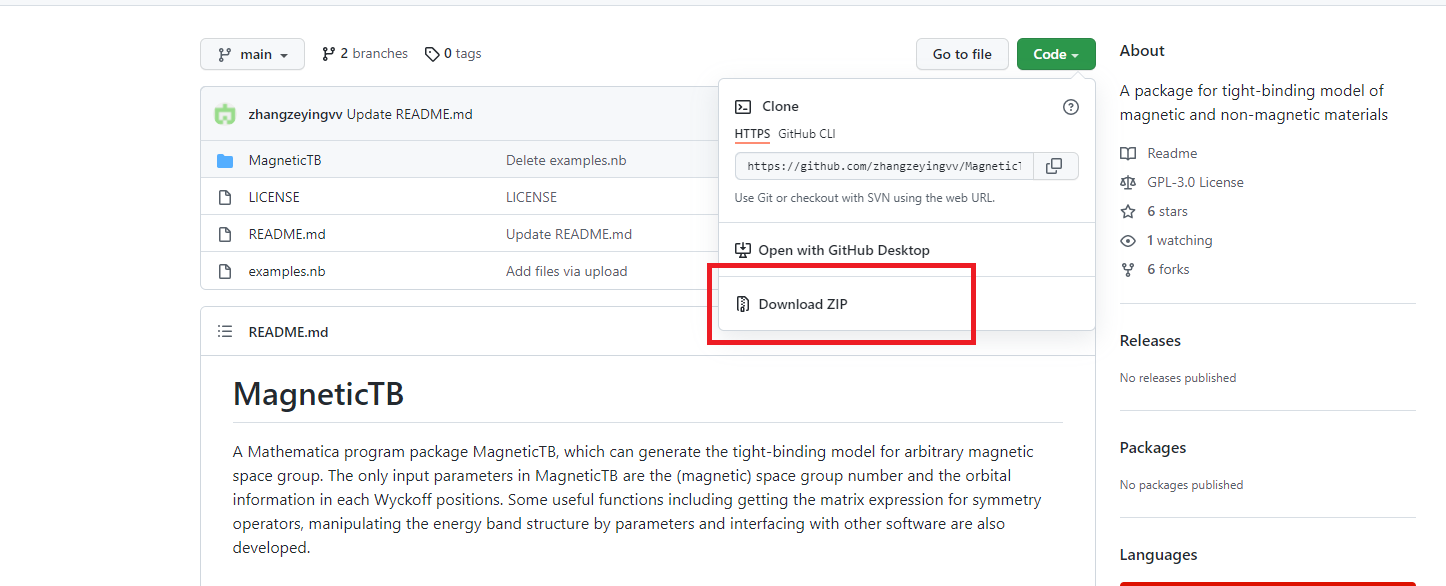
\includegraphics[width=1\textwidth]{./figures/安装1}
\end{figure}


打开Mathematica,运行:
\begin{lstlisting}[numbers=none]
$UserBaseDirectory
\end{lstlisting}
%\lstinline| $\mbox{\$}$ |
运行时点击Shift+回车。打开显示的目录,并进入Applications文件夹。

将刚刚下载的MagneticTB-main.zip解压,会得到一个MagneticTB文件夹和三个文件。把解压得到的MagneticTB文件夹复制到Applications文件夹内,安装完成。在Mathematica中运行
\begin{lstlisting}[numbers=none]
Needs["MagneticTB`"]
\end{lstlisting}	
即可载入程序包。
有经验的用户可以安装到\lstinline|$Path|中任何地方,部分目录需要管理员权限。以上方法对Windows和Linux用户均适用,也可参阅Comput. Phys. Commun.,
270,
108153 (2022)。

\section{使用方法}
\subsection{核心模块}
\textsf{MagneticTB}的核心功能是构造对称化的紧束缚模型。主要有三个函数构成,分别是\lstinline|msgop|, \lstinline|init|和\lstinline|symham|。

\lstinline|msgop|可以给出任意1651个磁群的对称操作,例如
\begin{lstlisting}
msgop[gray[191]]
msgop[bnsdict[{191, 236}]]
msgop[ogdict[{191, 8, 1470}]]
\end{lstlisting}	
第一行中\lstinline|gray[191]|为获取191号灰群(即为考虑时间反演对称性的空间群)的编码;
第二行中\lstinline|bnsdict[{191, 236}]|为获取BNS编号为$191.236$磁群的编码;
第三行中\lstinline|ogdict[{191, 8, 1470}]|为获取OG编号为$191.8.1470$磁群的编码;
用\lstinline|msgop[编码]|可获取对应磁群的对称操作,以上三条命令实际上是等价的,其输出为

\begin{lstlisting}
Magnetic space group (BNS): {191.234,P6/mmm1'}
Lattice: HexagonalP
Primitive Lattice Vactor: {{a,0,0},{-(a/2),(Sqrt[3] a)/2,0},{0,0,c}}
Conventional Lattice Vactor: {{a,0,0},{-(a/2),(Sqrt[3] a)/2,0},{0,0,c}}

{{"1",{{1,0,0},{0,1,0},{0,0,1}},{0,0,0},F},
{"6z",{{1,-1,0},{1,0,0},{0,0,1}},{0,0,0},F},
{"3z",{{0,-1,0},{1,-1,0},{0,0,1}},{0,0,0},F},
...
{"1",{{1,0,0},{0,1,0},{0,0,1}},{0,0,0},T},
{"6z",{{1,-1,0},{1,0,0},{0,0,1}},{0,0,0},T},
{"3z",{{0,-1,0},{1,-1,0},{0,0,1}},{0,0,0},T},
...}
\end{lstlisting}
1-4行为磁群的基本信息,包括符号、晶格类型和晶格矢量。6-13行为191号灰群的对称操作,1-4列分别为对称操作的名称、旋转部分、平移部分和是否包含时间反演操作。

有了对称操作就可以使用\lstinline|init|函数对结构进行初始化:
\begin{lstlisting}
sgop=msgop[gray[191]];
init[
	lattice -> {{a, 0, 0}, {-(a/2), (Sqrt[3] a)/2, 0}, {0, 0, c}},
	lattpar -> {a -> 1, c -> 3},
	wyckoffposition -> {{{1/3, 2/3, 0}, {0, 0, 0}}},
	symminformation -> sgop,
	basisFunctions -> {{"pz"}}];
\end{lstlisting}	
\lstinline|init|有五个选项必须设置(Mathematica中选项用一个横杠\lstinline|"-"|和一个大于号\lstinline|">"|连起来表示即\lstinline|"->"|),其中\lstinline|lattice|为晶格矢量和\lstinline|symminformation|为对称操作的集合可以直接使用\lstinline|msgop|的输出作为选项的值,也可以使用自己定义的对称操作。\lstinline|lattpar|为晶格矢量中参数的数值。\lstinline|wyckoffposition|为要考虑的Wyckoff点。其格式为:
\[
\{\{\boldsymbol{a}_{1},\boldsymbol{m}_{1}\},\{\boldsymbol{a}_{2},\boldsymbol{m}_{2}\},...\}
\]
$\boldsymbol{a}_{i}$和$\boldsymbol{m}_{i}$为第$i$个Wyckoff点的坐标和磁化方向。对于等价的Wyckoff点仅需输入其中任意一个即可。

\lstinline|basisFunctions|为每个Wyckoff点要考虑的基函数。其格式为:
\[
\{b_{1},b_{2},...\}
\]
$b_{i}$为第$i$个Wyckoff点要考虑的基函数列表。
其中基函数和字符串的对应关系如下表所示:
\begin{table}[H]
	\centering 
%\caption{\lstinline!basisFunctions!中原子轨道和字符串的对应关系}
	\label{tab:bf} %
	\begin{tabular}{cc|cc}
		\hline 
		基函数  & 代码  & 基函数  & 代码 \tabularnewline
		\hline 
		$s$  & \lstinline!"s"! & $p_{x}$  & \lstinline!"px"! \tabularnewline
		\hline 
		$p_{y}$  & \lstinline!"py"! & $p_{z}$  & \lstinline!"pz"! \tabularnewline
		\hline 
		$p_{x}+ip_{y}$  & \lstinline!"px+ipy"! & $p_{x}-ip_{y}$  & \lstinline!"px-ipy"! \tabularnewline
		\hline 
		$d_{z^{2}}$  & \lstinline!"dz2"! & $d_{xy}$  & \lstinline!"dxy"! \tabularnewline
		\hline 
		$d_{yz}$  & \lstinline!"dyz"! & $d_{xz}$  & \lstinline!"dxz"! \tabularnewline
		\hline 
		$d_{x^{2}-y^{2}}$  & \lstinline!"dx2-y2"!  &  & \tabularnewline
		\hline 
	\end{tabular}
\end{table}
\noindent 对于考虑自旋的情况,直接在代码后加\lstinline!"up"!或\lstinline!"dn"!。例如\lstinline!{"pzup","dxydn"}!。
如果遇到上表中没有的基函数,直接输入基函数的解析表达式也没问题,例如若想考虑$f_{xyz}$轨道,
直接输入\lstinline!basisFunctions -> {{x*y*z}}!。

在初始化函数运行完以后可以用\lstinline|atompos|检查一下生成的结构是否正确
\begin{lstlisting}
In:= atompos
Out:= {{{{1/3, 2/3, 0}, {0, 0, 0}}, {{2/3, 1/3, 0}, {0, 0, 0}}}}
\end{lstlisting}
表明该结构原胞中有两个要考虑的原子坐标为$(1/3,2/3,0)$和$(2/3,1/3,0)$。 \lstinline|{0, 0, 0}|为原子的磁化方向,在这里两个原子均没有磁性。运行完\lstinline!init!后可获取的基本性质如下表所示:
\begin{table}[ht]
	\centering
%	\caption{}
	\label{tab:pro} %
	\begin{tabular}{c|c}
		\hline 
		代码      & 性质说明 \tabularnewline
		\hline 
		\lstinline!atompos!  & 给出原胞中每个原子的原子坐标和磁化方向 \tabularnewline
		\hline 
		\lstinline!wcc!  & 给出每条轨道的中心 \tabularnewline
		\hline 
		\lstinline!reclatt!  & 倒格子 \tabularnewline
		\hline 
		\lstinline!symmetryops! & 对称操作的(共)表示矩阵 \tabularnewline
		\hline 
		\lstinline!unsymham[n]!  & 生成除平移对称性外没有任何对称性约束的$n-1$阶近邻的哈密顿量  \tabularnewline
		\hline
		\lstinline!symham[n]!  & 生成对称性约束的$n-1$阶近邻的哈密顿量  \tabularnewline
		\hline
		%		\hline \lstinline|symmetryopsII| 	& $P(Q)$ for each symmetry operator in conventions II (see Sec.~\ref{sec:IO})    \\
		%		\hline \lstinline|compactForm| 	& show matrix expression for $P(Q)$ and $Q$ in real space together    \\
		\lstinline!symmcompile!  & 给出对称操作、表示矩阵等信息 \tabularnewline
		\hline 
		\lstinline!bondclassify!  & 给出所有近邻的键长信息 \tabularnewline
		\hline
		\lstinline!showbonds[n]!  & 给出$n-1$阶近邻的键长信息 \tabularnewline
		\hline 
		%\lstinline!symham!  & generate the symmetry adopted Hamiltonian, see main text for detail \tabularnewline
		%\hline
	\end{tabular}
\end{table}

检查无误后就可以用\lstinline|symham[n]|生成考虑$n-1$近邻的的对称化紧束缚哈密顿量。例如
\begin{lstlisting}[numbers=none]
   symham[1]
\end{lstlisting}
会生成仅考虑在位能的哈密顿量。
\begin{lstlisting}[numbers=none]
Sum[symham[n], {n, 1, 3}];
\end{lstlisting}
会生成考虑在位能、最近邻和次近邻的哈密顿量。


\subsection{画图模块}
画图模块有两个函数 \lstinline|bandplot|和\lstinline|bandManipulate|。用法分别为
\begin{lstlisting}[numbers=none]
bandplot[能带路径, 每段能带中点的数目, symham生成的哈密顿量, 参数大小]
bandManipulate[能带路径, 每段能带中点的数目, symham生成的哈密顿量]
\end{lstlisting}
\lstinline|bandplot|可以画出较为美观的能带图,可以直接作为论文中的插图。\lstinline|bandManipulate|可以画出随参数大小动态显示的能带。具体例子见\ref{gra}。
\subsection{接口模块}
接口模块可以把\lstinline|symham|生成的哈密顿量转换为wannier90\_hr.dat格式的文件。用法为
\begin{lstlisting}[numbers=none]
hop[symham生成的哈密顿量,  参数大小]
\end{lstlisting}
具体例子见\ref{gra}。注意要用\lstinline|symham|生成的哈密顿量。\textbf{不要用自己化解后的哈密顿量作为输入,若想让某些参数等于$0$,直接在参数大小里指定某些参数为$0$。}

\subsection{能带表示模块}
能带表示模块可以计算紧束缚模型的能带表示。需要安装 \href{https://github.com/goodluck1982/SpaceGroupIrep}{\textsf{SpaceGroupIrep}} 和 \href{https://github.com/goodluck1982/MSGCorep}{\textsf{MSGCorep}} 软件包。能带表示模块主要有一下2个函数

\begin{lstlisting}[numbers=none]
	getMSGElemFromMSGCorep[{N1, N2}]
\end{lstlisting} 
从 \textsf{MSGCorep} 软件包中获取磁空间群元素,其中 N1.N2 是 BNS 磁空间群编号。
\begin{lstlisting}[numbers=none]
	getTBBandCorep[BNSNo, Hamiltonian, parameters, kset]
\end{lstlisting} 
给出紧束缚模型的共表示,其中 \lstinline!BNSNo! 是 BNS 磁空间群编号,\lstinline!Hamiltonian! 是由 \textsf{MagneticTB} 生成的哈密顿量,\lstinline!parameters! 是紧束缚模型中的参数,\lstinline!kset! 是包含多个 k 点的列表。

计算紧束缚能带表示的一般流程是
\begin{itemize}
	\item 使用 \lstinline!getMSGElemFromMSGCorep! (而不是\lstinline|msgop|)获取磁群元素和对应的晶格向量
	\item 用得到的磁群元素和对应的晶格向量结合自己设置 Wyckoff 位置和基函数构造紧束缚模型
	\item 用\lstinline!getTBBandCorep!获取能带表示
\end{itemize}
\section{例子}
\subsection{石墨烯}
\label{gra}
要生成石墨烯的费米面附近的紧束缚模型,仅需知道两个碳原子位于191号空间群的$2c$ Wyckoff点以及
费米面附近的电子态由碳原子的$p_z$轨道构成就足够了。
%用\textsf{MagneticTB}构造紧束缚模型。
具体代码如下:
\begin{lstlisting}
Needs["MagneticTB`"];
sgop = msgop[gray[191]];
init[
lattice -> {{a, 0, 0}, {-(a/2), (Sqrt[3] a)/2, 0}, {0, 0, c}},
lattpar -> {a -> 1, c -> 3},
wyckoffposition -> {{{1/3, 2/3, 0}, {0, 0, 0}}},
symminformation -> sgop,
basisFunctions -> {{"pz"}}];
ham = Sum[symham[i], {i, 3}]; 
MatrixForm[ham]
\end{lstlisting}
其中第1行为载入\textsf{MagneticTB}程序包;第2行为获取第191号灰空间群的对称操作;第3行为初始化函数;第4-8行为初始化函数的参数;第4行为晶格矢量;第5行为晶格常数中参数的数值;第6行为要考虑的Wyckoff点坐标和磁化方向;第7行为对称化紧束缚模型所满足的对称性;第8行为要考虑的原子轨道;第9行为输出考虑到次近邻的哈密顿量。
若要考虑自旋轨道耦合,仅需把第8行的
\begin{lstlisting}[numbers=none]
	basisFunctions -> {{"pz"}}];
\end{lstlisting}
改为
\begin{lstlisting}[numbers=none]
	basisFunctions -> {{"pzup","pzdn"}}];
\end{lstlisting}
即
\begin{lstlisting}[numbers=none]
sgop = msgop[gray[191]];
init[lattice -> {{a, 0, 0}, {-(a/2), (Sqrt[3] a)/2, 0}, {0, 0, c}}, 
lattpar -> {a -> 1, c -> 3}, 
wyckoffposition -> {{{1/3, 2/3, 0}, {0, 0, 0}}}, 
symminformation -> sgop,
basisFunctions -> {{"pzup", "pzdn"}}];
hamsoc = Sum[symham[i], {i, 3}]; 
MatrixForm[hamsoc]
\end{lstlisting}
就可以生成考虑自旋轨道耦合时的哈密顿量。得到哈密顿量后就可以画能带和生成wannier90\_hr.dat了。以下为画能带的具体代码:
\begin{lstlisting}
path={
	{{{0,0,0},{0,1/2,0}},{"G","M"}},
	{{{0,1/2,0},{1/3,1/3,0}},{"M","K"}},
	{{{1/3,1/3,0},{0,0,0}},{"K","G"}}
	};
bandManipulate[path, 20, ham]
bandplot[path, 200, ham, {e1 −> 0.05, t1 −> 0.5, r1−> 0}]
\end{lstlisting}
其中1-5行为定义$\boldsymbol{k}$点路径,第6行可以动态显示能带,第7行可以画出给定参数的能带。效果如下:
\begin{figure}[H]
	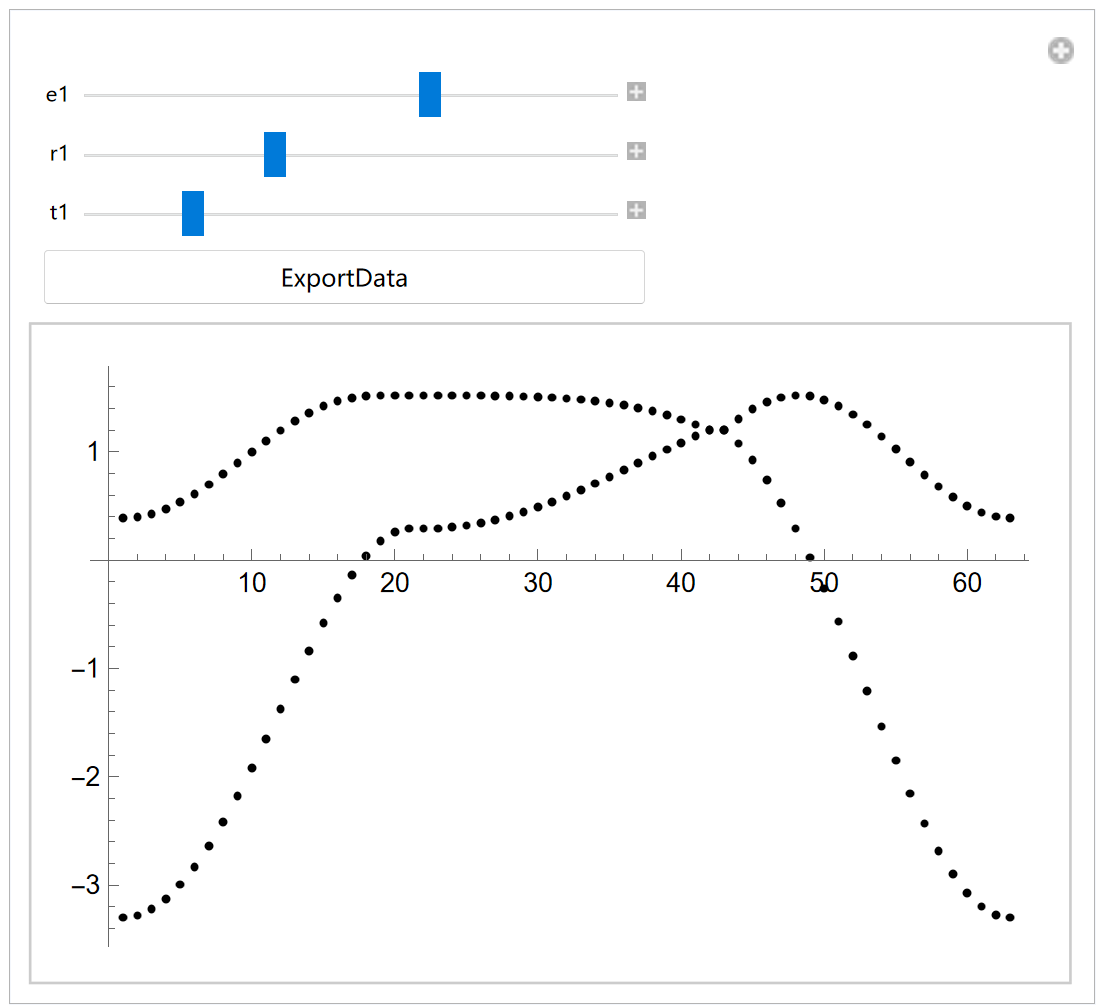
\includegraphics[width=.45\textwidth]{./figures/bm}
	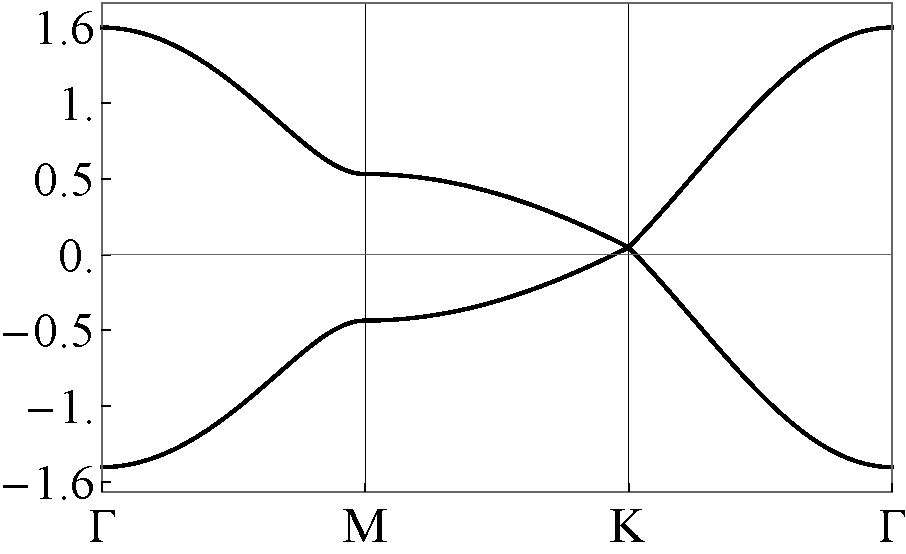
\includegraphics[width=.54\textwidth]{./figures/grabd}
\end{figure}
\noindent 可以点击“ExportData”显示参数的大小。


也可以用\lstinline|showbonds|查看石墨烯各个近邻之间的键长,例如查看次近邻键长用
\lstinline|showbonds[3]|,其输出为:
\begin{center}
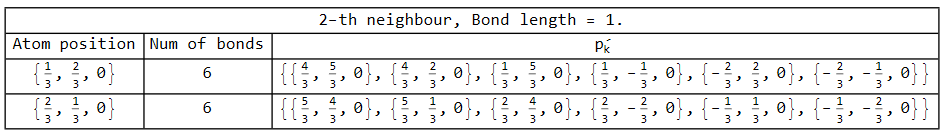
\includegraphics[width=1.0\textwidth]{./figures/showbonds.png}
\end{center}

要生成wannier90\_hr.dat,仅需运行以下命令:
\begin{lstlisting}[numbers=none]
hop[ham, {e1 -> 0, r1 -> 0.02,  t1 -> 0.5}]
\end{lstlisting}
其结果为:
\begin{lstlisting}[numbers=none]
Generated by MagneticTB
2
7
1    1    1    1    1    1    1
-1    -1     0     1     1    0.02000000    0.00000000
-1    -1     0     2     1    0.00000000    0.00000000
-1    -1     0     1     2    0.00000000    0.00000000
-1    -1     0     2     2    0.02000000    0.00000000
-1     0     0     1     1    0.02000000    0.00000000
-1     0     0     2     1    0.00000000    0.00000000
-1     0     0     1     2    0.50000000    0.00000000
-1     0     0     2     2    0.02000000    0.00000000
 0    -1     0     1     1    0.02000000    0.00000000
 0    -1     0     2     1    0.50000000    0.00000000
 0    -1     0     1     2    0.00000000    0.00000000
 0    -1     0     2     2    0.02000000    0.00000000
 0     0     0     1     1    0.00000000    0.00000000
 0     0     0     2     1    0.50000000    0.00000000
 0     0     0     1     2    0.50000000    0.00000000
 0     0     0     2     2    0.00000000    0.00000000
 0     1     0     1     1    0.02000000    0.00000000
 0     1     0     2     1    0.00000000    0.00000000
 0     1     0     1     2    0.50000000    0.00000000
 0     1     0     2     2    0.02000000    0.00000000
 1     0     0     1     1    0.02000000    0.00000000
 1     0     0     2     1    0.50000000    0.00000000
 1     0     0     1     2    0.00000000    0.00000000
 1     0     0     2     2    0.02000000    0.00000000
 1     1     0     1     1    0.02000000    0.00000000
 1     1     0     2     1    0.00000000    0.00000000
 1     1     0     1     2    0.00000000    0.00000000
 1     1     0     2     2    0.02000000    0.00000000
\end{lstlisting}

\subsection{更多例子}
更多例子请参阅example.nb文件。
\iffalse
\subsection{二硫化钼}

\begin{lstlisting}
sgop = msgop[gray[187]];
tran = {{1, -1, 0}, {0, 1, 0}, {0, 0, 1}};
sgoptr = MapAt[FullSimplify[tran . # . Inverse@tran] &, sgop, {;; , 2}];
init[
lattice -> {{1, 0, 0}, {1/2, Sqrt[3]/2, 0}, {0, 0, 100}},
lattpar -> {},
wyckoffposition -> {{{0, 0, 0}, {0, 0, 0}}},
symminformation -> sgoptr,
basisFunctions -> {{"dz2", "dxy", "dx2-y2"}}];
\end{lstlisting}

\subsection{磁性高阶节线相}
\begin{lstlisting}
sgop = msgop[bnsdict[{184, 196}]];
init[lattice -> {{Sqrt[3]/2, -( 1/2), 0}, {0, 1, 0}, {0, 0, 2}},
lattpar -> {},
wyckoffposition -> {{{0, 0, 0}, {0, 0, 1}}},
symminformation -> sgop,
basisFunctions -> {{{x + I y, 0}, {0, x - I y}}}]
\end{lstlisting}
\fi

\section{常见问题}
    \begin{enumerate}[style=nextline]
    \setlength\itemsep{1.5em}
	\litem{安装完以后运行没反应怎么办} 
	
	回答:仔细检查安装步骤,先把examples.nb文件中几个例子跑出来,实在不行在QQ群里提问。
	
	\litem{QQ群怎么加} 
	
	回答:群号为625192239。可以扫描以下二维码:
	\begin{figure}[H]
		\centering
		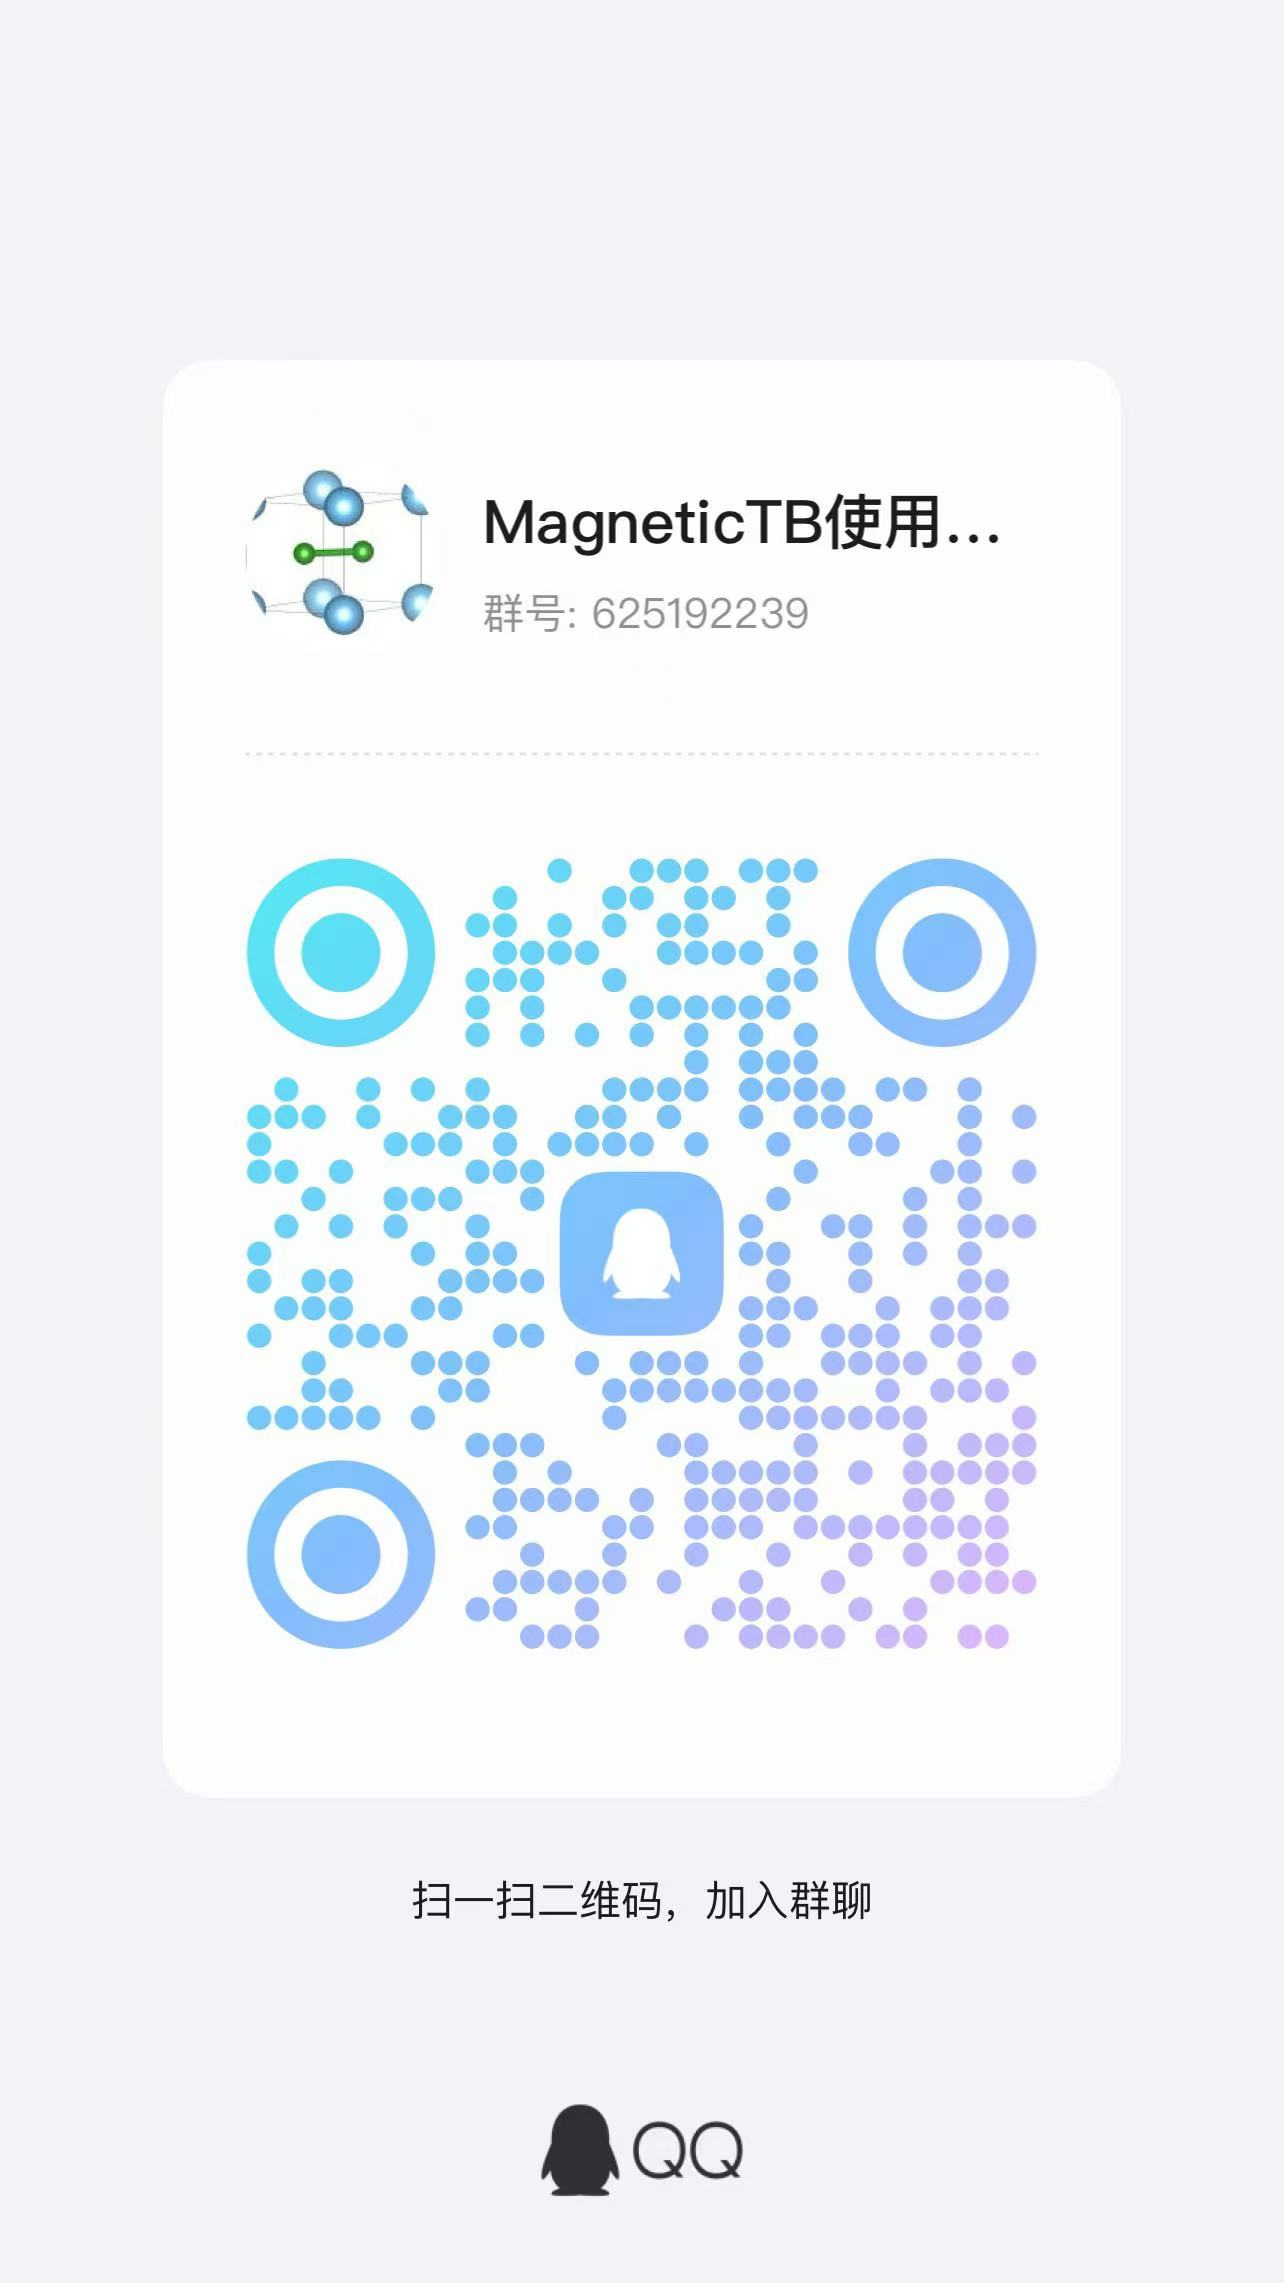
\includegraphics[width=.3\textwidth]{./figures/QQ}
	\end{figure}
	
	\litem{example.nb文件里二硫化钼的例子中的钼原子的Wyckoff点和BCS网站对不上,为什么}
	
	回答:这个例子是为了完全重复Phys. Rev. B 88, 085433 (2013) 的结果。数据库中默认的六角晶格$\boldsymbol{a}, \boldsymbol{b}$轴的夹角为$\frac{2\pi}{3}$。而Phys. Rev. B 88, 085433 (2013) 中使用的晶格矢量$\boldsymbol{a}, \boldsymbol{b}$轴的夹角为$\frac{\pi}{3}$。 所以为了保证对称操作与原包取法一致用\lstinline|sgoptr=MapAt[FullSimplify[tran . # . Inverse@tran] &, sgop, {;; , 2}]|把数据库中的对称操作转换了一下,得到的哈密顿量就与文献完全对上了。可以参考\textsf{SpaceGroupIrep}的文章Comput. Phys. Commun. 265, 107993  (2021)里说怎么具体转换。未来\textsf{MagneticTB}将集成自动转换功能。但是需要注意,不管原包的取法怎么变,最后得到的哈密顿量能带的简并和参数个数是一样的,仅会有形式上的不同。
	
	\litem{既然能算非磁性体系,为什么软件包叫\textsf{MagneticTB}}
	
	回答:因为230个空间群是1651个磁群的子集,\textsf{MagneticTB}可以构造任意1651个磁群的TB模型,包含了非磁性材料。
	

	
	\litem{我发现了Bug,该怎么办}
	
	回答:在QQ群里提问,在\url{https://github.com/zhangzeyingvv/MagneticTB/issues}上提问,给我发邮件zhangzeyingvv@gmail.com。
	
	\litem{除了想构造TB模型,我还算模型的拓扑性质,该怎么办}
	
	回答:\$UserBaseDirectory/MagneticTB/WilsonLoop.wl里有Wilson loop相关函数,可以参考,但该部分代码并未经过系统的测试,本文档不会提供Wilson loop相关函数使用方法。也可以将TB模型转换成wannier90\_hr.dat文件用其他软件算。
	
	
	\litem{\textsf{MagneticTB}支持构造自旋空间群的TB模型吗}

	回答:目前不支持,自旋空间群相关代码还在测试中,未来会发布。

	\litem{我又想考虑自旋,又不想考虑自旋轨道耦合,可以实现吗}
	
	回答:目前不行,更新了自旋空间群相关代码才能实现。

	\litem{有关于Mathematica的参考书吗}
	
	回答:推荐创造WOLFRAM语言的Wolfram本人写的《WOLFRAM  MATHEMATICA 实用编程指南》或《MATHEMATICA全书》。	
		
	\litem{可以转发该手册吗}

	回答:可以转发,同时如果想修改本手册,请通过github向我提issue(s)。

	\litem{如何引用\textsf{MagneticTB}}

    回答:Zeying Zhang, Zhi-Ming Yu, Gui-Bin Liu, Yugui Yao,
    Computer Physics Communications,
    270,
    108153 (2022).
    
    Bibtex:
    \begin{lstlisting}[numbers=none,language=TeX]
    	@article{ZHANG2022108153,
    		title = {MagneticTB: A package for tight-binding model of magnetic and non-magnetic materials},
    		journal = {Computer Physics Communications},
    		volume = {270},
    		pages = {108153},
    		year = {2022},
    		doi = {https://doi.org/10.1016/j.cpc.2021.108153},
    		url = {https://www.sciencedirect.com/science/article/pii/S0010465521002654},
    		author = {Zeying Zhang and Zhi-Ming Yu and Gui-Bin Liu and Yugui Yao}
    	}
    \end{lstlisting}
\end{enumerate}

\section{更新计划}
划线为已经完成的部分
\begin{itemize}
	\item	优化算法
%	\item   目前版本对于大体系仍然较慢,未来将优化约化参数的算法
	\item	将支持磁层群,磁杆群和自旋空间群
	\item	\sout{与\textsf{SpaceGroupIrep}和\textsf{MSGCorep}软件包接口}
	\item	\sout{增加拟合参数模块}
	\item	加入磁群的原点平移变换和晶格整体旋转变换
	\item	...
\end{itemize}





\end{document}
